\chapter{Modelliamo programmi}
\section{Un semplice linguaggio imperativo \texttt{IMP}}
Definiamo il linguaggio $\mathcal{L}$ dove:
\[
\begin{split}
    \mathbb{V} &= \mathbb{Z} \\
    \mathbb{X} &= \texttt{Var} \\
\end{split}
\]
\begin{grammar}
    <Exp $\mathbb{E}$> ::= $n\in \mathbb{V}$ | $x \in \mathbb{X}$ | 
    $\mathbb{E}  \oplus \mathbb{E}$

    <Bool $\mathbb{B}$> ::= \texttt{true} | \texttt{false} | $\mathbb{E} \oplus \mathbb{E}$

    <Com $\mathbb{C}$> ::= \texttt{skip} | $\mathbb{X} := \mathbb{E}$ | $\mathbb{C};\mathbb{C}$ |
    \texttt{if} $\mathbb{B}$ \texttt{then} $\mathbb{C}$ \texttt{else} $\mathbb{C}$
    \alt \texttt{while}  $\mathbb{B}$ | \texttt{input(x)} 

    <Programma $\mathbb{P}$> ::= $\mathbb{C}$
\end{grammar}
\subsection{La semantica di \texttt{IMP}}
La semantica è uno strumento formale che permette di dare significato ai programmi.


\begin{tcolorbox}[title = {Semantica operazionale}]
  La semantica operazionale è uno strumento formale che fornisce
  significato ai programmi attraverso la descrizione del comportamento
  passo dopo passo dell'interprete. Questo significa che il significato
  di un programma è descritto
  dalla sequenza dei singoli passi di computazione che esso compie.
\end{tcolorbox}

\begin{tcolorbox}[title = {Semantica denotazionale}]
  La semantica denotazionale attribuisce significato ai programmi
  tramite una funzione che associa a ciascun programma un valore.
  In termini matematici, possiamo rappresentare questa idea come segue:
    \[
      \texttt{intput}  \xrightarrow[\text{semantica}]{} \texttt{output} 
    \]
  In altre parole, esiste una funzione $\llbracket . \rrbracket$ che
  mappa l'input del programma all'output. Questa approccio è composito,
  il che significa che possiamo definire il significato di programmi
  composti in termini dei loro componenti, come segue:
    \[
      \llbracket . \rrbracket   : \texttt{intput}  \rightarrow \texttt{output}
    \]
    \[
      \llbracket P_1; P_2\rrbracket  = \llbracket P_2\rrbracket  \oplus \llbracket P_1\rrbracket
    \]
\end{tcolorbox}
Queste due forme di semantica, operazionale e denotazionale, sono
strumenti utili per comprendere
il significato dei programmi in modo dettagliato e matematico.
\subsection{Lo stato della memoria}
Nel contesto della programmazione, lo ``stato" rappresenta una
fotografia istantanea della configurazione della macchina (\textit{astratta})
su cui viene eseguito un programma. Questo stato descrive l'associazione
tra le variabili del programma e i valori che contengono. Formalmente,
possiamo rappresentare lo stato come una funzione $\mathbb{M}$ che
mappa le variabili ($\mathbb{X}$) ai loro valori ($\mathbb{V}$), come
segue:
\[
  \mathbb{M} : \mathbb{X} \rightarrow \mathbb{V}
\]
Durante l'esecuzione di un programma, viene generata una sequenza di
stati che riflettono come il programma modifica lo stato della memoria
nel corso del tempo. Questa sequenza di stati è essenziale per
comprendere come il programma funziona e come influisce sullo stato
della macchina. Nel contesto della modellazione formale, spesso ci
riferiamo a questo processo come ``esecuzione".

Per descrivere l'evoluzione di uno stato durante l'esecuzione di
un programma, utilizziamo un modello chiamato ``sistema di transizione",
che è rappresentato da una coppia $\langle \Sigma, \rightarrow \rangle$.
In questa coppia, $\Sigma$ rappresenta l'insieme degli stati possibili
e $\rightarrow$ rappresenta la relazione che specifica come un
determinato stato può transizionare in un altro stato a seguito
dell'esecuzione di un'azione del programma. Questo modello è
fondamentale per analizzare il comportamento dinamico di un programma
e comprendere come le modifiche di stato si verificano nel corso
dell'esecuzione.
\subsection{Semantica delle transizioni di stato}

La semantica è definita come l'insieme di tutte le possibili sequenze
di transizioni di stato (\textit{eventualmente infinite}) a partire dagli stati
iniziali, ovvero le esecuzioni delle istruzioni di un programma,
indicate da sequenze di stati nel sistema di transizione.

Fornisce il significato dei programmi attraverso l'esecuzione delle
loro istruzioni su un interprete (\textit{cioè componendo gli effetti delle
istruzioni}).

Il modello matematico si basa sull'utilizzo delle tracce in un sistema
di transizione.

\subsection{Semantica delle espressioni}

La semantica delle espressioni è definita come segue:
\[
\llbracket E \rrbracket : \mathbb{M} \rightarrow \mathbb{V}
\]
a partire dalla memoria in $\mathbb{M}$ restituisce:

\subsubsection{Valori}

Il valore in $\mathbb{V}$ rappresentato da $e$. In altre parole:
\[
m\in \mathbb{M}\quad, n \in \mathbb{V}
\]
\[
\llbracket n \rrbracket (m) = n
\]
\[
\llbracket x \rrbracket (m) = m(x)
\]
Quindi, per un'espressione composta:
\[
\llbracket e_1 \oplus e_2 \rrbracket (m) = f_{\oplus}(\llbracket e_1 \rrbracket (m), \llbracket e_2 \rrbracket (m) )
\]

Dove il simbolo $\oplus$ è il simbolo sintattico e $f_{\oplus}$ è la funzione semantica.

\subsubsection{Booleani}

Per i valori booleani:
\[
b \in \mathbb{B} \qquad \llbracket tt \rrbracket (m) = tt \qquad \llbracket ff \rrbracket( m )= ff
\]
\[
\llbracket b_1 \oplus b_2 \rrbracket (m) = f_{\oplus}(\llbracket b_1 \rrbracket (m), \llbracket b_2 \rrbracket (m) )  
\]

\subsection{Semantica dei comandi}

La semantica dei comandi è definita come segue:
\[
c \in \mathbb{C}. \quad \llbracket c \rrbracket : \mathbb{M} \rightarrow \mathbb{M}
\]

\subsubsection{\texttt{skip}}

L'istruzione \texttt{skip} rappresenta un comando nullo che non modifica lo stato della memoria.
\[
\llbracket \texttt{skip} \rrbracket (m) = m
\]

\subsubsection{Composizione}

La composizione di due comandi $c_1$ e $c_2$ esegue prima $c_1$ e poi $c_2$. La semantica della composizione è data da:
\[
\llbracket c_1; c_2 \rrbracket (m) = \llbracket c_2 \rrbracket (\llbracket c_1 \rrbracket (m)) = \llbracket c_2 \rrbracket \oplus \llbracket c_1 \rrbracket (m)
\]

\subsubsection{Assegnamento}

L'assegnamento dell'espressione $e$ alla variabile $x$ modifica lo stato della memoria mappando $x$ al valore di $e$ in $m$.
\[
\llbracket x := e \rrbracket (m) = m[x \mapsto \llbracket e \rrbracket (m)]
\]

\subsubsection{\texttt{input}}

L'istruzione \texttt{input(x)} rappresenta l'input di un valore
$n$ nella variabile $x$ all'interno dello stato della memoria $m$.
\[
\llbracket \texttt{input(x)} \rrbracket (m) = m[x \mapsto n] 
\quad n \in \mathbb{V}
\]

\subsubsection{If-then-else}

L'istruzione condizionale \texttt{if b then c_1 else c_2} esegue $c_1$
se la condizione $b$ è vera, altrimenti esegue $c_2$.
\[
\llbracket \texttt{if} \quad b \quad \texttt{then} \quad c_1 \quad \texttt{else} \quad c_2 \rrbracket (m) = 
\begin{cases}
\llbracket c_1 \rrbracket (m) & \text{se } \llbracket b \rrbracket
(m) = \texttt{true} \\
\llbracket c_2 \rrbracket (m) & \text{se } \llbracket b \rrbracket
(m) = \texttt{false} \\
\end{cases}
\]

\subsubsection{While}

L'istruzione \texttt{while b do c} rappresenta un ciclo che continua
a eseguire $c$ fintanto che la condizione $b$ è vera. La semantica di
\texttt{while} è definita come segue:
\[
\llbracket \texttt{while} \quad b \quad \texttt{do} \quad c
\rrbracket (m) =
\begin{cases}
\llbracket \texttt{while} \quad b \quad \texttt{do} \quad c
\rrbracket (\llbracket c \rrbracket (m)) & \text{se } \llbracket b
\rrbracket (m) = \texttt{true} \\
m & \text{se } \llbracket b \rrbracket (m) = \texttt{false} \\
\end{cases}
\]

Il while può comportare un ciclo infinito. Per gestire questa
eventualità, si utilizza il concetto di traccia del programma e il
punto di programma, raccogliendo gli stati raggiunti fino a quel punto.
Questo permette di lavorare con proprietà degli input invece di
manipolare singoli valori, affrontando problemi legati all'infinito.
\section{Semantica Transazionale}

La semantica transazionale è un approccio alla comprensione del
comportamento dei programmi attraverso la raccolta e l'analisi delle
tracce di esecuzione. Questo approccio considera l'insieme di tutte
le tracce di esecuzione possibili, partendo dagli stati iniziali del
programma. Questa raccolta di tracce è nota come ``program trace
semantics" (\textit{semantica delle tracce di programma}).

Le tracce di programma forniscono una visione dettagliata
dell'evoluzione del programma nel tempo, inclusi gli stati intermedi
e le transizioni tra di essi. Questa analisi delle tracce è preziosa
per comprendere come il programma risponde a diverse condizioni e
input, e può rivelare informazioni importanti sul suo comportamento
dinamico.

La semantica transazionale è particolarmente utile per affrontare
problemi legati all'infinito, in quanto consente di lavorare con
tracce e punti di programma invece di manipolare singoli valori.
Questo approccio facilita la gestione delle esecuzioni potenzialmente
infinite, fornendo una base solida per l'analisi formale dei programmi.

Nel complesso, la semantica transazionale fornisce uno strumento potente
per la comprensione approfondita del comportamento dei programmi,
evidenziando le variazioni nello stato della memoria nel corso
dell'esecuzione e consentendo l'analisi delle proprietà attraverso
l'osservazione delle tracce di programma.
\begin{figure}[H]
  \centering 
  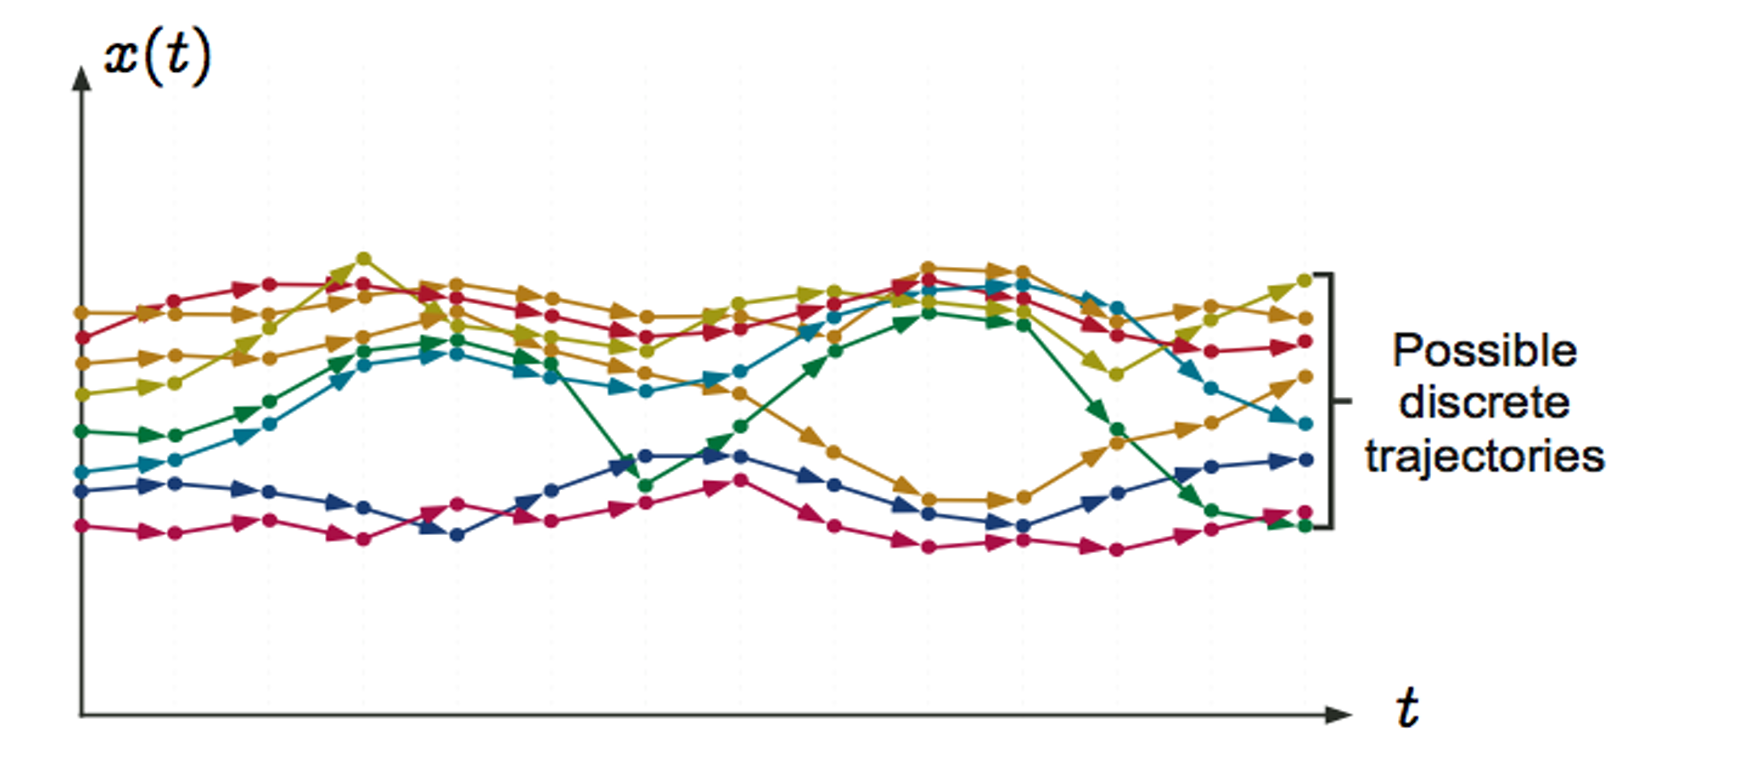
\includegraphics[scale=0.5]{img/collezionetacce.png}
\end{figure}

\section{Semantica come punto fisso}
\begin{tcolorbox}[title={Semantica a punto fisso}]
  Dato un dominio $D$ di stati e una funzione $F$:
  \begin{itemize}
  \item $D$ è un ordine parziale, cioè $\langle D, \leq \rangle$ è un \textit{po-set}, dove $D$ soddisfa le seguenti proprietà:
  \begin{itemize}
      \item Riflessività: $\forall x \in D: x \leq x$.
      \item Antisimmetria: $\forall x, y \in D: (x \leq y \land y \leq x) \Rightarrow x = y$.
      \item Transitività: $\forall x, y, z \in D: (x \leq y \land y \leq z) \Rightarrow x \leq z$.
  \end{itemize}
  \item $F: D \rightarrow D$ è una funzione totale e monotona, il che significa che per ogni $x$ e $y$ in $D$ se $x \leq y$, allora $F(x) \leq F(y)$. Inoltre, la funzione $F$ è iterabile, cioè può essere composta con se stessa più volte, ottenendo $F^n(x) = F(F(F(\ldots F(x)))$.
  \end{itemize}
  \end{tcolorbox}
  
  Un sistema di transizione è una coppia $\langle \Sigma, \tau \rangle$, dove $\Sigma$ è un insieme non vuoto di stati e $\tau$ è una relazione di transizione che collega gli stati. In altre parole, un sistema di transizione rappresenta un insieme di stati e le relazioni tra di essi, ed è utilizzato per descrivere il comportamento di sistemi o programmi.
\subsection{Punto fisso inferiore}
\begin{itemize}
  \item Il punto rosso \textcolor{red}{$\odot$} rappresenta un stato 
  bloccato.
  \item Il punto blu \textcolor{blue}{$\bullet$} rappresenta uno stato
  non bloccato.
\end{itemize}
Quindi, possiamo rappresentare l'evoluzione del sistema attraverso iterazioni. Iniziamo con un insieme vuoto di stati $X^0$:
Nella prima iterazione, otteniamo l'insieme $X^1$ contenente uno stato bloccato:

\[
  X^0 = \varnothing
\]
Nella prima iterazione, otteniamo l'insieme $X^1$ contenente uno stato bloccato:
\[
  X^1 = \{\textcolor{red}{\odot} \} 
\]
Nella seconda iterazione, aggiungiamo uno stato non bloccato con una transizione $\tau$ dall'insieme $X^1$ all'insieme $X^2$:
\[
  X^2 = \{\textcolor{red}{\odot}, \textcolor{blue}{\bullet}\xrightarrow[]{\tau} \textcolor{red}{\odot} \} 
  \qquad \text{dove } \{\textcolor{red}{\odot}\} \cup \textcolor{blue}{\bullet}\xrightarrow[]{\tau}\{ \textcolor{red}{\odot}\}
\]
In questa iterazione, uno stato non bloccato può avanzare diventando uno stato bloccato. La notazione $\textcolor{blue}{\bullet}\xrightarrow[]{\tau}$ indica una transizione che può verificarsi.
Nella terza iterazione, continuiamo ad aggiungere stati e transizioni:
Qui vediamo che gli stati non bloccati possono ancora avanzare tramite transizioni $\tau$, ma alla fine possono diventare stati bloccati.

Tutti gli stati contenuti in $X^3$ rappresentano gli stati terminati del sistema, ossia quegli stati in cui il sistema non può avanzare ulteriormente.

Qui vediamo che gli stati non bloccati possono ancora avanzare tramite
transizioni $\tau$, ma alla fine possono diventare stati bloccati.

Tutti gli stati contenuti in $X^3$ rappresentano gli stati terminati
del sistema, ossia quelli in cui il sistema non può avanzare ulteriormente.

La notazione finale, $\textit{lfp}^{\subseteq}_{\varnothing}F^+$,
rappresenta il calcolo del punto fisso inferiore di una funzione o di
un operatore $F$ in questo contesto. In questo calcolo, stiamo cercando
il più piccolo insieme di stati che rimane invariato quando applichiamo
l'operatore $F$ iterativamente a partire da un insieme vuoto. Questo è
fondamentale per identificare gli stati stabili o terminali in un sistema
o un processo.
\subsection{Punto fisso superiore}
\begin{itemize}
  \item Il punto rosso \textcolor{red}{$\odot$} rappresenta uno stato
  bloccato.
  \item Il punto blu \textcolor{blue}{$\bullet$} rappresenta uno stato
  non bloccato.
  \item Il punto arancione \textcolor{orange}{$\bullet$} rappresenta uno
  stato non bloccato che può avanzare e diventare uno stato bloccato.
\end{itemize}
Ora, possiamo rappresentare l'evoluzione del sistema attraverso
iterazioni. Iniziamo con un insieme iniziale $X^0$ che contiene
uno stato non bloccato che può avanzare e diventare uno stato bloccato, con un 
numero di passi non definito:
\[
  X^0 = \{ \textcolor{orange}{\bullet}, \textcolor{orange}{\bullet} \xrightarrow[]{?}\textcolor{orange}{\bullet},
  \textcolor{orange}{\bullet} \xrightarrow[]{?}\textcolor{orange}{\bullet}\xrightarrow[]{?}\textcolor{orange}{\bullet},
  \dots,
  \textcolor{orange}{\bullet} \xrightarrow[]{?}\textcolor{orange}{\bullet}
  \dots
  \textcolor{orange}{\bullet} \xrightarrow[]{?}\textcolor{orange}{\bullet}
  ,\dots\}
\]
Nella prima iterazione, otteniamo l'insieme $X^1$, che include uno stato
bloccato e uno stato non bloccato che può avanzare tramite una transizione
$\tau$:

\[
  X^1 = \{ \textcolor{red}{\odot}, \textcolor{blue}{\bullet} \xrightarrow[]{\tau}\textcolor{orange}{\bullet},
  \textcolor{blue}{\bullet} \xrightarrow[]{\tau}\textcolor{orange}{\bullet}\xrightarrow[]{?}\textcolor{orange}{\bullet},
  \dots,
  \textcolor{blue}{\bullet} \xrightarrow[]{\tau}\textcolor{orange}{\bullet}
  \dots
  \textcolor{orange}{\bullet} \xrightarrow[]{?}\textcolor{orange}{\bullet}
  ,\dots\}
\]
Nella seconda iterazione, otteniamo l'insieme $X^2$, che include uno
stato bloccato, uno stato non bloccato che può avanzare tramite una
transizione $\tau$, e uno stato non bloccato che può continuare a
evolversi:
\[
  X^2 = \{ \textcolor{red}{\odot}, \textcolor{blue}{\bullet} \xrightarrow[]{\tau}\textcolor{red}{\odot},
  \textcolor{blue}{\bullet} \xrightarrow[]{\tau}\textcolor{blue}{\bullet} \xrightarrow[]{\tau}\textcolor{orange}{\bullet},
  \dots,
  \textcolor{blue}{\bullet} \xrightarrow[]{\tau}\textcolor{blue}{\bullet} \xrightarrow[]{\tau}
  \textcolor{orange}{\bullet}
  \dots
  \textcolor{orange}{\bullet} \xrightarrow[]{?}\textcolor{orange}{\bullet}
  ,\dots\}
\]
Qui vediamo che gli stati non bloccati possono avanzare tramite transizioni $\tau$, ma alla fine possono diventare stati bloccati.

L'insieme $\{\textcolor{red}{\odot}\} \cup \textcolor{blue}{\bullet}\xrightarrow[]
{\tau} \Sigma^{+}$ rappresenta il punto fisso superiore
(\textit{gfp}) in questo contesto. Il \textit{gfp} rappresenta il
più grande insieme di stati che rimane invariato quando applichiamo
l'operatore $\Sigma^{+}$ iterativamente a partire da un insieme
vuoto. In altre parole, è l'insieme più grande in cui gli stati
non bloccati possono continuare a evolversi. Il \textit{gfp} è
fondamentale per identificare gli stati stabili o terminali in un
sistema o un processo.
\[
  \textit{gfp}^{\subseteq}_{\Sigma^\omega}F^\omega
\]

\subsection{Semantica dei comandi come punto fisso}
La semantica dei comandi mappa un insieme di input in un 
insieme di stati.
\[
  \llbracket \mathbb{C} \rrbracket_\wp : \wp{P}(\mathbb{M}) \rightarrow \wp(\mathbb{M})
\]
\[
  \llbracket \texttt{skip} \rrbracket_\wp(M) = M
\]
\[
  \llbracket {C_0;C_1} \rrbracket_\wp(M) = \llbracket {C_1} \rrbracket_\wp(\llbracket {C_0} \rrbracket_\wp(M))
\]
\[
  \llbracket {\texttt{x:= E}} \rrbracket_\wp(M) = \{m[x \mapsto \llbracket {E} \rrbracket_M(m)] \mid m \in M\}
\]
\[
  \llbracket \texttt{input(x)} \rrbracket_\wp(M) = \{m[x \mapsto n] \mid m \in M, n \in \mathbb{V}\}
\]
\[
  \llbracket {\texttt{if B then C else C'}} \rrbracket_\wp(M) = \llbracket C_0 \rrbracket_\wp 
  (\mathcal{F}_B (M)) \cup \llbracket C_1 \rrbracket_\wp (\mathcal{F}_{\neg B} (M))
\]
\[
  \llbracket {\texttt{while B do C}} \rrbracket_\wp(M) = \mathcal{F}_{\neg B}
  \left ( \bigcup_{i \geq 0}(\llbracket C \rrbracket_\wp \circ 
  \mathcal{F}_B)^i (M)\right )
\]
Dove:
\[
  \mathcal{F}_B(M)= \{m \in M | 
  \llbracket B \rrbracket (m) = \texttt{true}\}
\]
\subsubsection{Semantica del ciclo}
Dobbiamo partizionare l'esecuzione basandola sul numero di iterazioni
che il ciclo esegue prima di uscire.
L'insieme degli output è l'infinita unione della famiglia di insiemi $M_i$
che denotano gli stati prodotti dal programma in esecuzione.
\[
  M_i = \mathcal{F}_{\neg B}\left ( (\llbracket C \rrbracket_\wp \circ \mathcal{F}_B)^i (M)\right )
\]
Dove:
\[
\bigcup_{i \geq 0}M_i = \bigcup_{i\geq 0} \mathcal{F}_{\neg B}\left ( (\llbracket C \rrbracket_\wp \circ \mathcal{F}_B)^i (M)\right )
= \mathcal{F}_{\neg B}\left ( \bigcup_{i \geq 0}(\llbracket C \rrbracket_\wp \circ \mathcal{F}_B)^i (M)\right )
\]
Notiamo che:
\[
  \mathcal{F}_{\neg B}(\textit{lfp}_M F) \textit{ dove }F : M' \mapsto M \cup \llbracket C \rrbracket_\wp  \circ (\mathcal{F}_B(M'))
\]
